\chapter {Analyzer}

Analyzer's role is to provide a facade over objects and methods to create a simple interface for processing --- analyzing --- a single HLASM source file. The output of the analysis is data for LSP server.

\section{Overview}

\begin{figure}
	\centering
	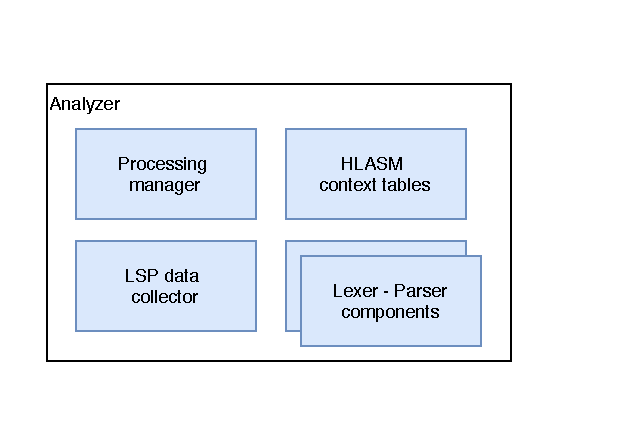
\includegraphics[width=\textwidth / 2]{img/analyzer_arch}
	\caption{The composition of the Analyzer component}
	\label{fig06:analyzer}
\end{figure}

Analyzer is composed of several sub-components, all required to properly process the file (see \cref{fig06:analyzer}). 
\begin{itemize}
	\item \emph{LSP data collector} collects and retieves all LSP information created while processing the file.
	\item \emph{HLASM context tables} hold information about the context of processed HLASM source code.
	\item Analyzer contains several \emph{Lexer - Parser sub-components} to simplify the processing interface and ease the use of this component.
	\item \emph{Processing manager} executes the main loop where file is processed.
\end{itemize}

LSP data collector is required by Lexer-Parser sub-components that are required by processing manager. HLASM context tables are used by the manager and the sub-components as well.

\subsection{Construction}

In order to parse a HLASM file, analyzer is constructed with the following parameters:
\begin{itemize}
	\item \emph{Name and content of the file}
	\item \emph{Parse library provider} -- object responsible for resolving source file dependencies. The dependencies are only discovered during the analysis, so it is not possible to provide the files beforehand.
	\item \emph{Processing tracer} (see \cref{chap:macro_tracer}).
\end{itemize}

When this constructor is used, analyzer creates HLASM context tables and processes the provided source as an open-code. We say that analyzer has \emph{owner semantics}. 
 
Analyzer provides \emph{reference semantics} as well. The provided source is not treated as an open-code, rather as an external file dependency. The constructor of an analyzer with reference semantics adds two parameters to the previous one:
\begin{itemize}
	\item \emph{HLASM context tables reference} -- belonging to the owning open-code analyzer.
	\item \emph{Library data} -- states how the dependency file should be treated (see \cref{lab06:lib_data}).
\end{itemize}

This constructor is called within open-code analyzer by it's sub-components when they use \emph{Parse library provider}.

\vspace{0.5cm}

To sum up, after analyzer is constructed, it analyses provided source file. As result, it updates HLASM context tables and provides a list of diagnostics linked to the file, highlighting, list of symbol definitions, etc.

\section{LSP data collector}

The data collection is necessary to be able to reply to the LSP requests without the need to re-parse. During the parsing process, the component called \emph{LSP info processor} processes and stores this information. The main goal of this component is to collect as much information as possible to provide meaningful and complex replies to the LSP requests while maintaining the memory and parse-time overhead negligible.

\emph{LSP info processor} is invoked after each parsed and processed statement to collect and store the information it needs inside the \emph{LSP context} (part of HLASM context). 

We will describe the component in better detail as a cross product of distinct symbols and the LSP features. Possible LSP features are:
\begin{enumerate}
	\item \emph{hover}
	\item \emph{complete}
	\item \emph{go\_to\_definition}
	\item \emph{references}
\end{enumerate}
The symbols, on which the user might call mentioned LSP feautures, are:
\begin{enumerate}
	\item \emph{instructions}
	\item \emph{variable symbols}
	\item \emph{sequence symbols}
	\item \emph{ordinary symbols}
\end{enumerate}

The \emph{references} feature uses the same symbols as \emph{go\_to\_definition}, its usage is straightforward and therefore does nothing that needs to be further explained.

\subsection{Instructions}

The most complex symbols are instructions. To be able to provide information about each built-in instruction, we extract its type and parameters from the checker component (\cref{checker}).

As we know, user defined macros are instructions as well. These are added to the list of all instructions after their first use in the open code. Macros can also be redefined in the open code, resulting in distinct macros with same name being used across the open code.

The \emph{hover} feature displays the instruction's type, the syntax of its parameters and, in case of macros, its version and documentation. The \emph{go\_to\_definition} works only in case of macros and goes to the definition of the macro.

Whenever a user types an A-Z character after arbitrary number of whitespaces from the left side, the \emph{complete} for instructions is issued. This rolls out a list of all possible instructions with the information about them similar to the \emph{hover}.

\subsection{Variable Symbols}

Variable symbols are used in substitutions and begin with \& (\cref{var_sym}). Based on the instruction that have set the variable symbol, it may be of type \emph{number}, \emph{string} or \emph{bool}, which is displayed on both \emph{hover} and \emph{complete}. Those variable symbols that are declared as macro parameters (and therefore have no type) are labeled as \emph{Macro Param}.

The \emph{complete} is triggered whenever user types \& and responds with list of variable symbols that have been defined so far.

The \emph{go\_to\_definition} jumps to the first occurence of the symbol.

\subsection{Sequence Symbols}

Probably the most interesting information about the sequence symbols is their position, which is also the displayed information for both \emph{hover} and \emph{complete}.

The \emph{complete} is triggered whenever user types . and responds with list of sequence symbols that have been defined so far.

The \emph{go\_to\_definition} jumps to the target destination of the sequence symbol, i.e. where will the "jump" take the code generation.

\subsection{Ordinary Symbols}

Ordinary symbols have the capability to hand over various information about the code. They are also the only symbols for which only the name placeholders with their positions are collected after each processed statement. After the parsing, these placeholders are matched with their values, accordingly to the ordinary processor (\cref{ord_proc}). \emph{COPY} instruction's parameter is also considered an ordinary symbol in LSP context.  

The \emph{go\_to\_definition} either jumps to the definition of the ordinary symbol which is a label or, in case of COPY parameter, to the file where the COPY is defined.

The \emph{hover} gives information whether the symbol is absolute or not, its value and its attributes values. 




